\documentclass[12pt]{article}
\usepackage{geometry}                % See geometry.pdf to learn the layout options. There are lots.
\geometry{letterpaper}                   % ... or a4paper or a5paper or ... 
%\geometry{landscape}                % Activate for for rotated page geometry
%\usepackage[parfill]{parskip}    % Activate to begin paragraphs with an empty line rather than an indent
\usepackage{graphicx}
\usepackage{amssymb}
\usepackage{subfig}
\usepackage{multirow}
\usepackage{pstricks,pst-node,pst-tree}



\title{Analysis of loadings}
\author{Wesley Brooks}
\date{}                                           % Activate to display a given date or no date

\usepackage{Sweave}
\begin{document}
\setkeys{Gin}{width=0.9\textwidth}    %make figures a bit wider than the Sweave default.
\maketitle


\section{Introduction}
Minimizing the erosion of sediment into streams is a goal for water quality managers. In order to develop plans to limit the amount of sediment that gets into streams, those managers need to know how sediment gets into the water. A recent study \cite{Danz:2010} has shown that 

The next block of code produces a set of bar charts that show the relative contributions of the snow-driven events, post-snow-pre-vegetation events, and the post-vegetation events.\\





\section{Variable selection}
In order to make a model of the load carried by the stream, we need to select the predictor variables that have explanatory power. We use stepwise regression with the Bayesian Information Criterion (BIC) to screen the potential predictor variables.


\begin{table}[h]
    \begin{center}
    \begin{tabular}{lrl}
        Solids: & & \\
        & Eagle & theisen, antecedent\_qbase, p15max, p60max\\
        & Joos & theisen, antecedent\_qbase, p15max, ap\_2day\\
        & Otter & theisen, antecedent\_qbase, antecedent\_tmean, julian\\
        & Brewery & theisen, p30max, tmean\\
        \hline \\
        Phosphorus: & & \\
        & Eagle & theisen, antecedent\_qbase, tmean, tmax, p15max, p30max\\
        & Joos & theisen, antecedent\_qbase, p15max, ap\_2day\\
        & Otter & theisen, antecedent\_qbase, tmean, julian\\
        & Brewery & theisen, p30max, tmean, ap\_3day\\
    \end{tabular}
    \end{center}
\end{table}



\begin{Schunk}
\begin{Soutput}
Call:
lm(formula = log_stot_tot ~ antecedent_qbase + theisen, data = eagle_nosnow)

Residuals:
     Min       1Q   Median       3Q      Max 
-1.36985 -0.38539 -0.01636  0.36174  1.72769 

Coefficients:
                 Estimate Std. Error t value Pr(>|t|)    
(Intercept)      -1.35345    0.09295  -14.56   <2e-16 ***
antecedent_qbase  0.15791    0.00996   15.86   <2e-16 ***
theisen           0.86034    0.04071   21.13   <2e-16 ***
---
Signif. codes:  0 ‘***’ 0.001 ‘**’ 0.01 ‘*’ 0.05 ‘.’ 0.1 ‘ ’ 1 

Residual standard error: 0.5152 on 242 degrees of freedom
  (2 observations deleted due to missingness)
Multiple R-squared: 0.7554,	Adjusted R-squared: 0.7534 
F-statistic: 373.8 on 2 and 242 DF,  p-value: < 2.2e-16 
\end{Soutput}
\begin{Soutput}
Call:
lm(formula = log_stot_tot ~ antecedent_qbase + theisen, data = joosvalley_nosnow)

Residuals:
     Min       1Q   Median       3Q      Max 
-2.53840 -0.37911 -0.02301  0.32260  1.91902 

Coefficients:
                 Estimate Std. Error t value Pr(>|t|)    
(Intercept)      -1.34618    0.08411  -16.01   <2e-16 ***
antecedent_qbase  0.19763    0.01717   11.51   <2e-16 ***
theisen           0.85938    0.04357   19.72   <2e-16 ***
---
Signif. codes:  0 ‘***’ 0.001 ‘**’ 0.01 ‘*’ 0.05 ‘.’ 0.1 ‘ ’ 1 

Residual standard error: 0.5812 on 251 degrees of freedom
  (3 observations deleted due to missingness)
Multiple R-squared: 0.6647,	Adjusted R-squared: 0.662 
F-statistic: 248.8 on 2 and 251 DF,  p-value: < 2.2e-16 
\end{Soutput}
\begin{Soutput}
Call:
lm(formula = log_stot_tot ~ antecedent_qbase + theisen, data = otter_nosnow)

Residuals:
    Min      1Q  Median      3Q     Max 
-1.3252 -0.2519 -0.0092  0.2702  1.3771 

Coefficients:
                  Estimate Std. Error t value Pr(>|t|)    
(Intercept)      -1.379094   0.054726  -25.20   <2e-16 ***
antecedent_qbase  0.121272   0.007881   15.39   <2e-16 ***
theisen           0.934789   0.046258   20.21   <2e-16 ***
---
Signif. codes:  0 ‘***’ 0.001 ‘**’ 0.01 ‘*’ 0.05 ‘.’ 0.1 ‘ ’ 1 

Residual standard error: 0.4372 on 245 degrees of freedom
  (2 observations deleted due to missingness)
Multiple R-squared: 0.7385,	Adjusted R-squared: 0.7363 
F-statistic: 345.9 on 2 and 245 DF,  p-value: < 2.2e-16 
\end{Soutput}
\begin{Soutput}
Call:
lm(formula = log_stot_tot ~ antecedent_qbase + theisen, data = brewery_nosnow)

Residuals:
    Min      1Q  Median      3Q     Max 
-2.1064 -0.5225  0.1222  0.4687  1.7584 

Coefficients:
                 Estimate Std. Error t value Pr(>|t|)    
(Intercept)      -0.44937    0.19369  -2.320   0.0216 *  
antecedent_qbase -0.07398    0.08070  -0.917   0.3606    
theisen           0.69205    0.06874  10.068   <2e-16 ***
---
Signif. codes:  0 ‘***’ 0.001 ‘**’ 0.01 ‘*’ 0.05 ‘.’ 0.1 ‘ ’ 1 

Residual standard error: 0.7512 on 161 degrees of freedom
  (128 observations deleted due to missingness)
Multiple R-squared: 0.3884,	Adjusted R-squared: 0.3808 
F-statistic: 51.13 on 2 and 161 DF,  p-value: < 2.2e-16 
\end{Soutput}
\begin{Soutput}
Call:
lm(formula = log_ptot_tot ~ antecedent_qbase + theisen, data = eagle_nosnow)

Residuals:
     Min       1Q   Median       3Q      Max 
-0.98156 -0.23430  0.00308  0.20073  1.46374 

Coefficients:
                  Estimate Std. Error t value Pr(>|t|)    
(Intercept)      -0.145134   0.067172  -2.161   0.0317 *  
antecedent_qbase  0.108446   0.007198  15.067   <2e-16 ***
theisen           0.714547   0.029420  24.288   <2e-16 ***
---
Signif. codes:  0 ‘***’ 0.001 ‘**’ 0.01 ‘*’ 0.05 ‘.’ 0.1 ‘ ’ 1 

Residual standard error: 0.3723 on 242 degrees of freedom
  (2 observations deleted due to missingness)
Multiple R-squared: 0.7826,	Adjusted R-squared: 0.7808 
F-statistic: 435.6 on 2 and 242 DF,  p-value: < 2.2e-16 
\end{Soutput}
\begin{Soutput}
Call:
lm(formula = log_ptot_tot ~ antecedent_qbase + theisen, data = joosvalley_nosnow)

Residuals:
     Min       1Q   Median       3Q      Max 
-1.82432 -0.22751 -0.04278  0.20511  1.72563 

Coefficients:
                 Estimate Std. Error t value Pr(>|t|)    
(Intercept)      -0.26036    0.06052  -4.302 2.43e-05 ***
antecedent_qbase  0.15271    0.01236  12.356  < 2e-16 ***
theisen           0.70562    0.03136  22.504  < 2e-16 ***
---
Signif. codes:  0 ‘***’ 0.001 ‘**’ 0.01 ‘*’ 0.05 ‘.’ 0.1 ‘ ’ 1 

Residual standard error: 0.4182 on 251 degrees of freedom
  (3 observations deleted due to missingness)
Multiple R-squared: 0.7151,	Adjusted R-squared: 0.7128 
F-statistic:   315 on 2 and 251 DF,  p-value: < 2.2e-16 
\end{Soutput}
\begin{Soutput}
Call:
lm(formula = log_ptot_tot ~ antecedent_qbase + theisen, data = otter_nosnow)

Residuals:
     Min       1Q   Median       3Q      Max 
-0.99166 -0.25833  0.01595  0.27079  1.03556 

Coefficients:
                  Estimate Std. Error t value Pr(>|t|)    
(Intercept)      -0.045816   0.046203  -0.992    0.322    
antecedent_qbase  0.102279   0.006653  15.372   <2e-16 ***
theisen           0.783261   0.039054  20.056   <2e-16 ***
---
Signif. codes:  0 ‘***’ 0.001 ‘**’ 0.01 ‘*’ 0.05 ‘.’ 0.1 ‘ ’ 1 

Residual standard error: 0.3691 on 245 degrees of freedom
  (2 observations deleted due to missingness)
Multiple R-squared: 0.7365,	Adjusted R-squared: 0.7344 
F-statistic: 342.4 on 2 and 245 DF,  p-value: < 2.2e-16 
\end{Soutput}
\begin{Soutput}
Call:
lm(formula = log_ptot_tot ~ antecedent_qbase + theisen, data = brewery_nosnow)

Residuals:
     Min       1Q   Median       3Q      Max 
-1.46780 -0.31817  0.02745  0.28340  1.34380 

Coefficients:
                 Estimate Std. Error t value Pr(>|t|)    
(Intercept)       0.55719    0.12465   4.470 1.47e-05 ***
antecedent_qbase -0.10602    0.05193  -2.041   0.0428 *  
theisen           0.69750    0.04424  15.767  < 2e-16 ***
---
Signif. codes:  0 ‘***’ 0.001 ‘**’ 0.01 ‘*’ 0.05 ‘.’ 0.1 ‘ ’ 1 

Residual standard error: 0.4834 on 161 degrees of freedom
  (128 observations deleted due to missingness)
Multiple R-squared: 0.6111,	Adjusted R-squared: 0.6062 
F-statistic: 126.5 on 2 and 161 DF,  p-value: < 2.2e-16 
\end{Soutput}
\end{Schunk}










The next block prints a table of the proportion of total phosphorus loading due to each class of event at each site\\


% latex table generated in R 2.13.0 by xtable 1.5-6 package
% Thu Aug  4 13:20:15 2011
\begin{table}[h]
\begin{center}
\begin{tabular}{lccc}
  & snowmelt-driven & early post-snow & late post-snow \\ 
  \hline
eagle & 27.0\% & 29.1\% & 43.9\% \\ 
  joosvalley & 26.9\% & 20.5\% & 52.6\% \\ 
  otter & 35.4\% & 20.5\% & 44.1\% \\ 
  brewery & 32.8\% & 4.5\% & 62.7\% \\ 
  \end{tabular}
\caption{Proportion of total suspended solids loading contributed by each type of event}
\label{tab:stot}
\end{center}
\end{table}
% latex table generated in R 2.13.0 by xtable 1.5-6 package
% Thu Aug  4 13:20:15 2011
\begin{table}[h]
\begin{center}
\begin{tabular}{lccc}
  & snowmelt-driven & early post-snow & late post-snow \\ 
  \hline
eagle & 32.8\% & 22.9\% & 44.2\% \\ 
  joosvalley & 36.4\% & 16.9\% & 46.7\% \\ 
  otter & 46.5\% & 16.6\% & 36.9\% \\ 
  brewery & 49.6\% & 4.5\% & 45.9\% \\ 
  \end{tabular}
\caption{Proportion of total phosphorus loading contributed by each type of event}
\label{tab:ptot}
\end{center}
\end{table}










Produce plots of the proportion of the suspended solids and phosphorus (both total loading and stormflow loading) that is contributed by each class of event at each stream site:\\



\begin{figure}[h!]
    \begin{center}
\includegraphics{loadings-fig2}
    \end{center}
    \vspace{-10mm}
    \caption{Cumulative storm loadings at the four creeks.\label{bars}}
\end{figure}












%Boxplots of the contribution from individual storm events
\begin{figure}[h]
    \setkeys{Gin}{width=1\textwidth}    %make figures a bit wider than the Sweave default.
    \begin{center}
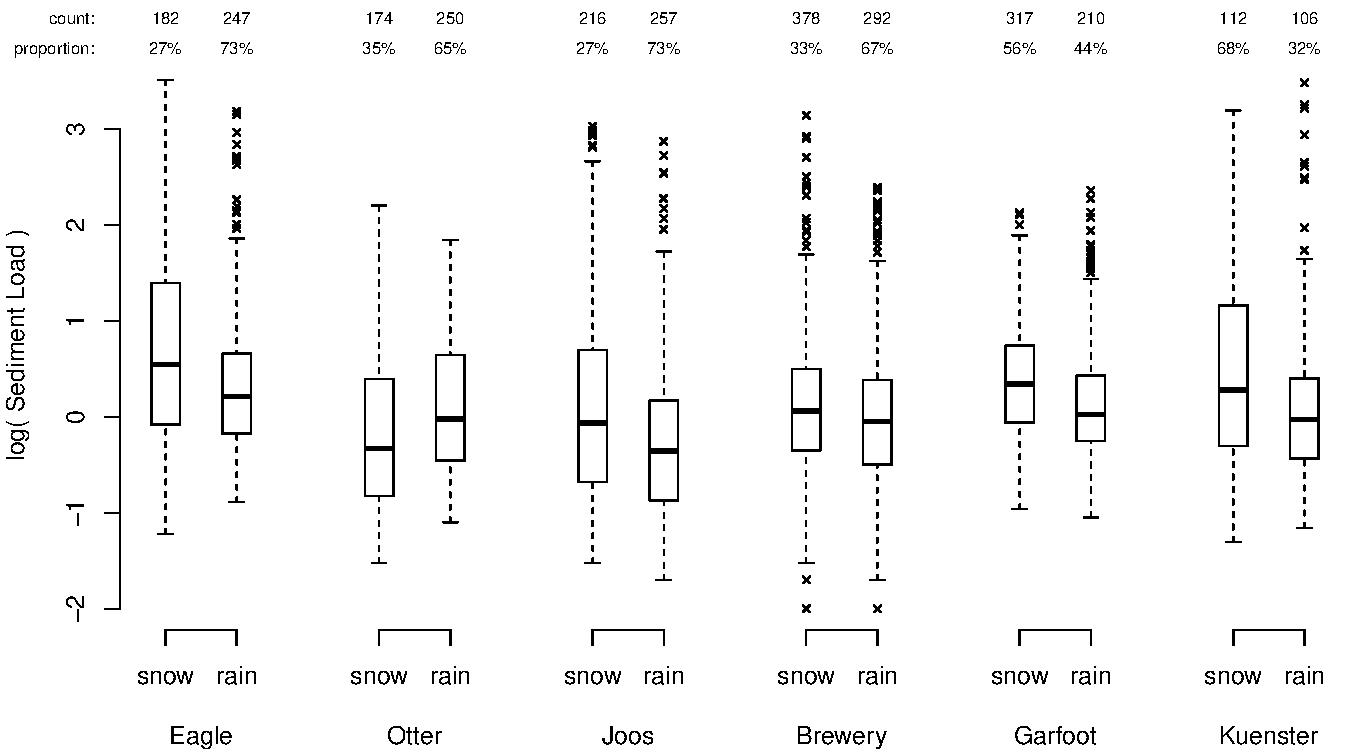
\includegraphics{loadings-boxplot_stot}
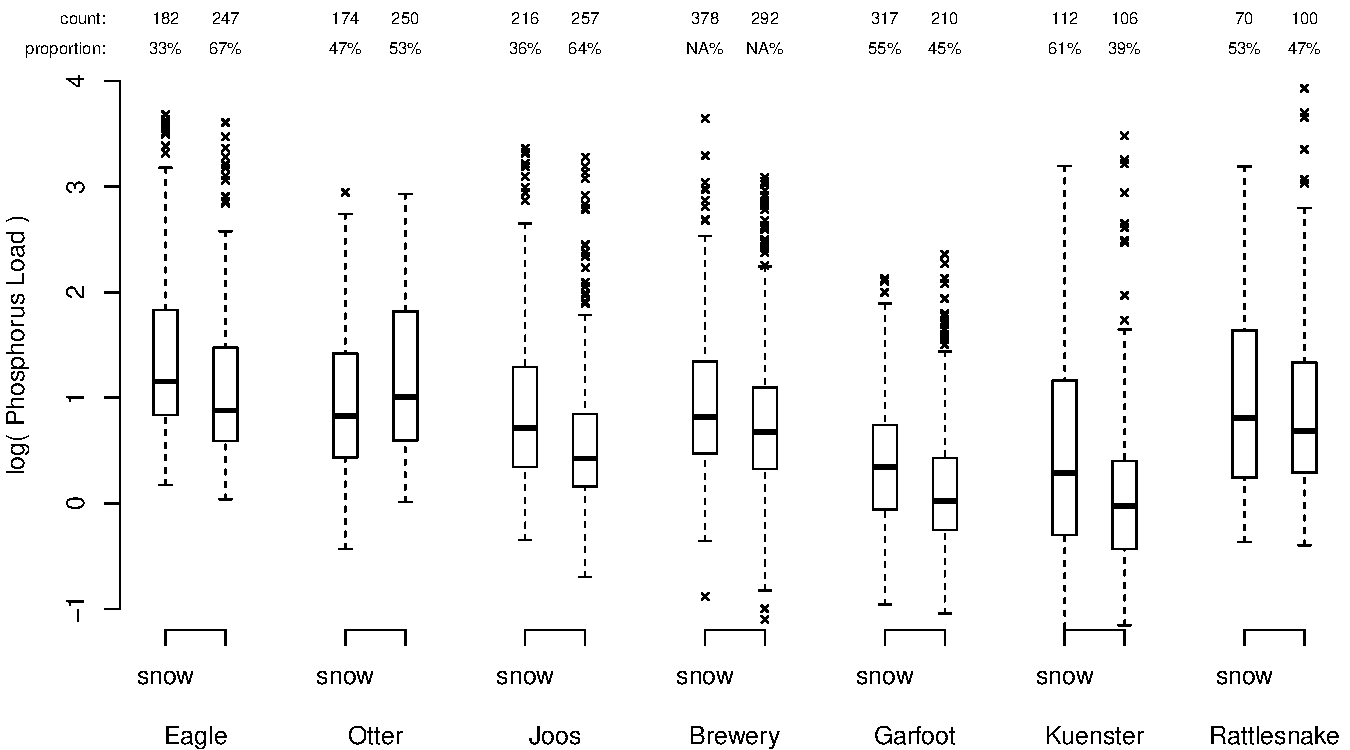
\includegraphics{loadings-boxplot_ptot}
    \end{center}
\end{figure}










\begin{figure}
    \begin{center}
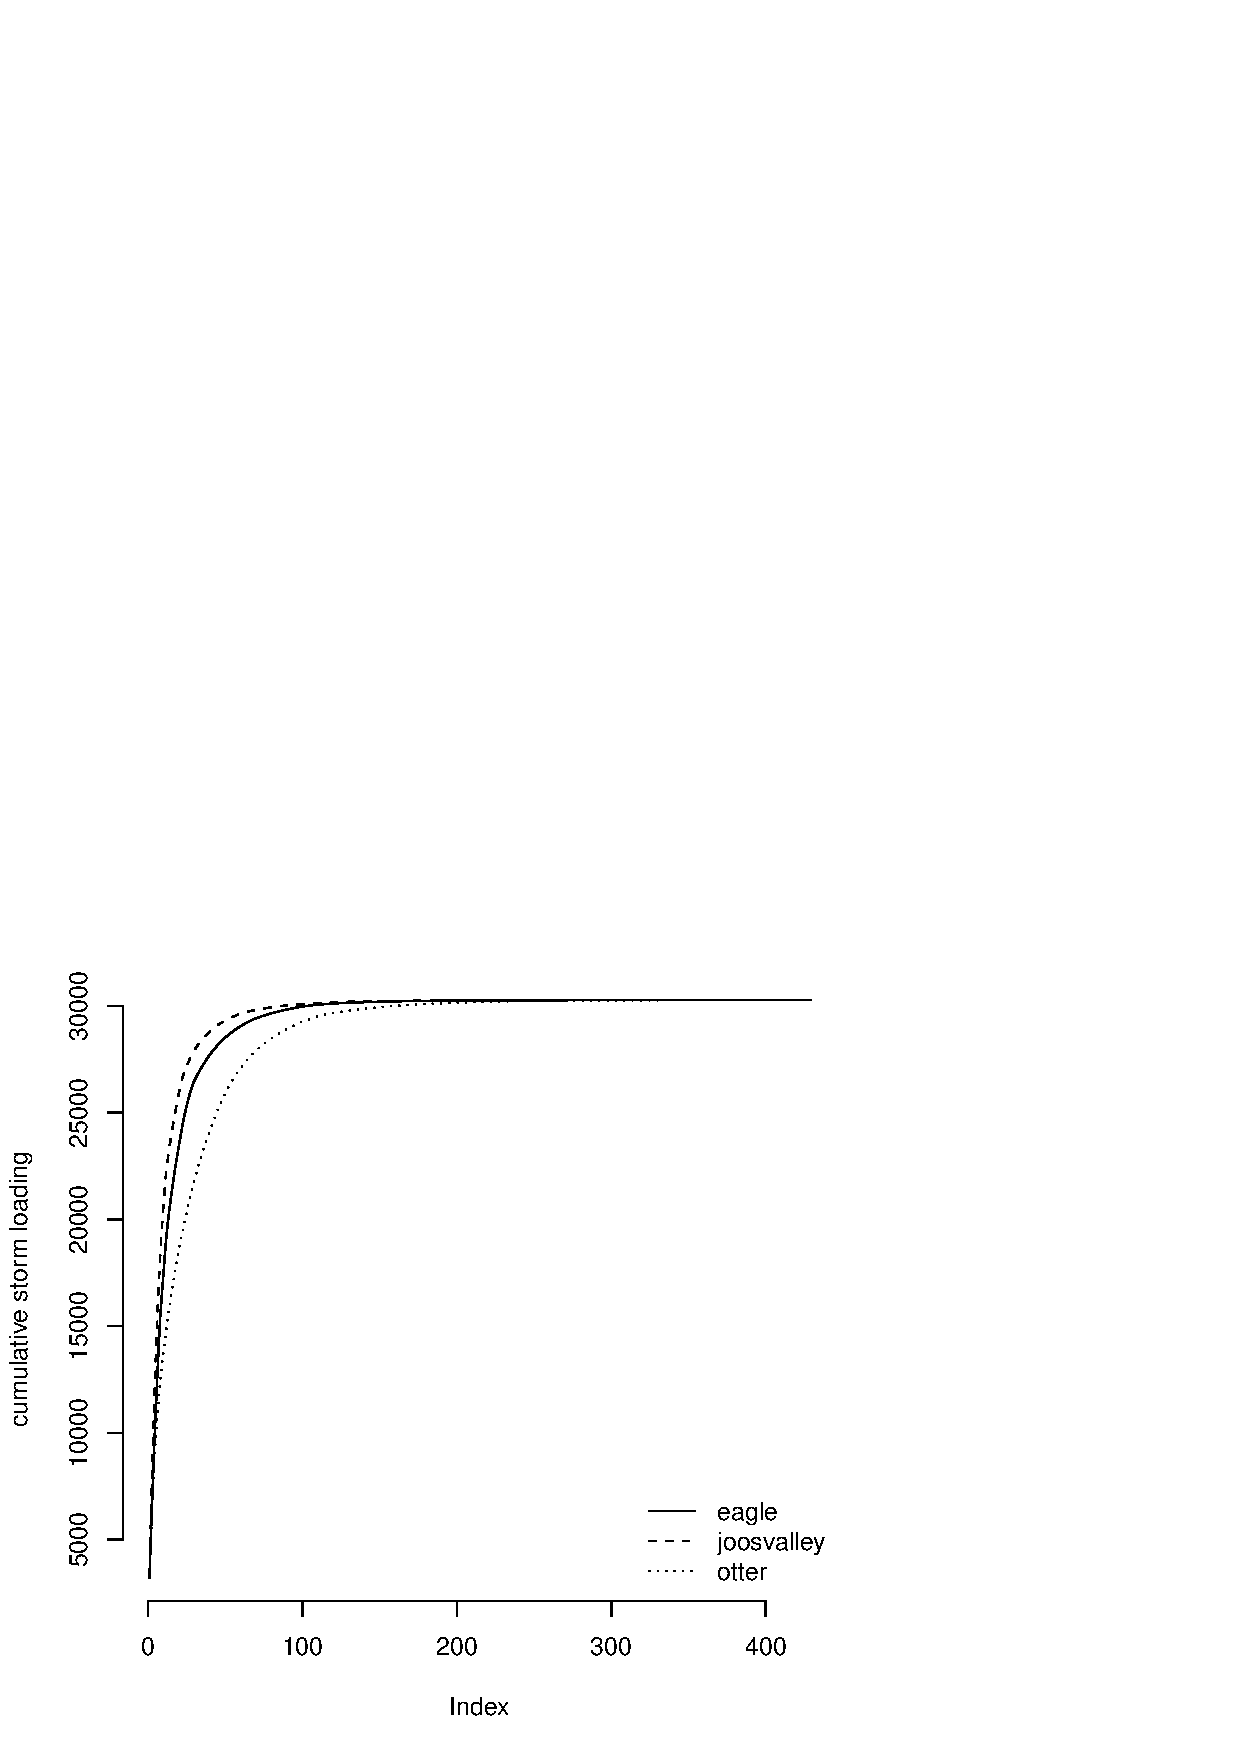
\includegraphics{loadings-figure1}
    \end{center}
    \caption{Cumulative storm loadings at the three creeks.\label{cdf}}
\end{figure}


\begin{figure}
    \begin{center}
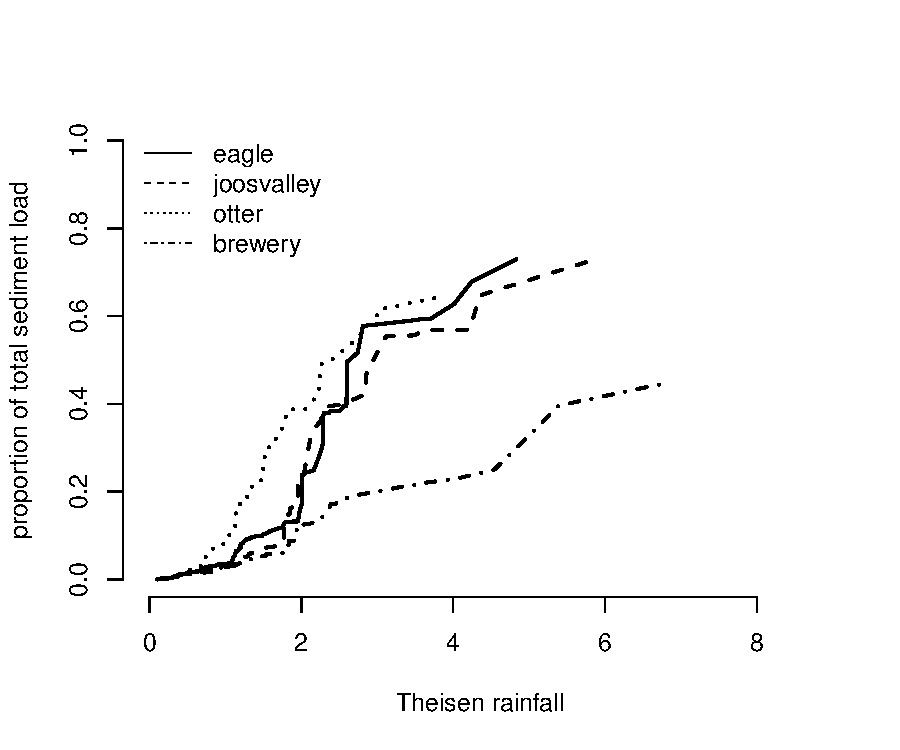
\includegraphics{loadings-figure2}
    \end{center}
    \caption{Proportion of the total sediment load contributed by rainfall events up to the size shown. Snowmelt-driven events are excluded.\label{cdf-p}}
\end{figure}

\begin{figure}
    \begin{center}
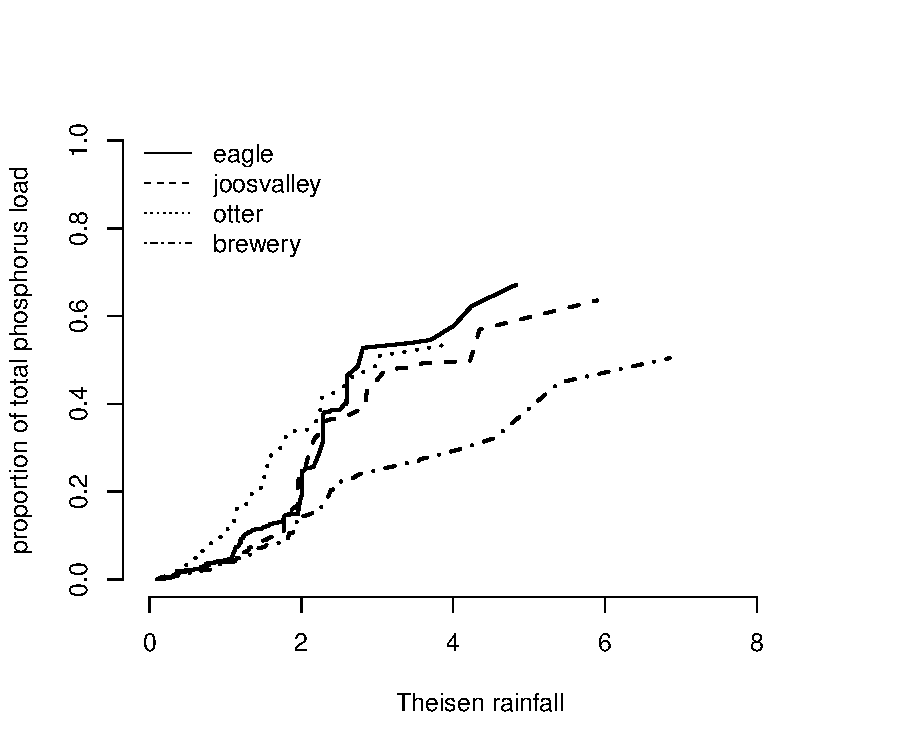
\includegraphics{loadings-figure3}
    \end{center}
    \caption{Proportion of the total phosphorus load contributed by rainfall events up to the size shown. Snowmelt-driven events are excluded.\label{cdf-s}}
\end{figure}



Figure out what proportion of total sediment loading is contributed by the top 10\% of storms:\\








The top 10\% of events contributed 89.1\% of the sediment loading at Eagle Creek, 73.1\% of the sediment loading at Otter Creek, 93.4\% of the sediment loading at Joos Valley Creek, and 90.4\% of the sediment loading at Joos Valley Creek.\\

Now we want to know how these major events are distributed within the event classes; that is, whether snowmelt tends to produce major loading events, or whether it is the post-snow events. Note that the \_tot column measures the total loading during an event. The snowmelt-driven events are different in kind than the rainfall-driven ones because they don't require continuous rain during the event. If the snowmelt-driven events are caused by warm weather, it seems reasonable that a single event might last for many days and cause more loading than a more-intense rainfall event that only lasts a day or two. To account for this, we will look both at total loading (\_tot) and average daily loading during an event (\_avg).\\


\begin{table}[h]
    \begin{center}
    \begin{tabular}{lr|lr|lr|l}
        & \multicolumn{2}{c}{Snowmelt    }\ & \multicolumn{2}{c}{Early post-snow}\ & \multicolumn{2}{c}{Late post-snow} \\
        Creek & All & Major & All & Major & All & Major \\
        \hline 
        Eagle & 42\% & 30\% & 13\% & 19\% & 45\% & 51\% \\
        Otter & 41\% & 42\% & 11\% & 19\% & 48\% & 40\% \\
        Joos & 46\% & 31\% & 11\% & 17\% & 43\% & 52\% \\
        
        Brewery & 56\% & 52\% & 6\% & 6\% & 38\% & 42\% \\
        
    \end{tabular}
    \end{center}
\end{table}



The table shows that the major loading events that produce the majority of the loading can be occur during each of the three annual periods. However, the events caused by snowmelt produced a smaller proportion of major events than their proportion of all events, and their relative contribution to the total sediment load was smaller than their proportion of loading events. Taken together, these insights tell us that, while snowmelt can cause a major loading event, a snowmelt-driven event is less likely to be a major contributor to sediment load than is a rainfall-driven event.\\



\begin{table}[h]
    \begin{center}
    \begin{tabular}{llccccc}
        &  &  & \multicolumn{2}{c}{Sediment} & \multicolumn{2}{c}{Phosphorus} \\
        Creek & Period & All events & Major events & Loading & Major events & Loading \\
        \hline 
        \multirow{3}{*}{Aggregated} & Snowmelt & 
        48\% &
        28\% & 
        40\% & 
        39\% & 
        48\% \\
        & Early post-snow & 
        10\% &
        23\% & 
        14\% & 
        17\% & 
        13\% \\
        & Late post-snow & 
        43\% &
        49\% & 
        46\% & 
        44\% & 
        39\% \\
        
        \hline 
        \multirow{3}{*}{Eagle} & Snowmelt & 
        42\% &
        27\% & 
        30\% & 
        33\% & 
        37\% \\
        & Early post-snow & 
        13\% &
        29\% & 
        19\% & 
        23\% & 
        21\% \\
        & Late post-snow & 
        45\% &
        44\% & 
        51\% & 
        44\% & 
        42\% \\
        
        \hline 
        \multirow{3}{*}{Joos} & Snowmelt & 
        46\% &
        27\% & 
        31\% & 
        36\% & 
        35\% \\
        & Early post-snow & 
        11\% &
        20\% & 
        17\% & 
        17\% & 
        19\% \\
        & Late post-snow & 
        43\% &
        53\% & 
        52\% & 
        47\% & 
        46\% \\
        
        \hline 
        \multirow{3}{*}{Otter} & Snowmelt & 
        41\% &
        35\% & 
        42\% & 
        47\% & 
        58\% \\
        & Early post-snow & 
        11\% &
        20\% & 
        19\% & 
        17\% & 
        12\% \\
        & Late post-snow & 
        48\% &
        44\% & 
        40\% & 
        37\% & 
        30\% \\
        
        \hline 
        \multirow{3}{*}{Brewery} & Snowmelt & 
        56\% &
        33\% & 
        52\% & 
        50\% & 
        60\% \\
        & Early post-snow & 
        6\% &
        5\% & 
        6\% & 
        5\% & 
        4\% \\
        & Late post-snow & 
        38\% &
        63\% & 
        42\% & 
        46\% & 
        37\% \\
    \end{tabular}
    \end{center}
\end{table}



 %\begin{landscape}
 \begin{center}
\psset{linecolor=black,tnsep=2pt,tnheight=0cm,treesep=.3cm,levelsep=40pt,radius=10pt}
%     \def\psedge#1#2{\ncangle{#2}{#1}}
%     \pstree[treemode=R]
    \Tcircle[fillcolor=yellow,fillstyle=solid]{ 1 }~{\textit{48.34}}
 \end{center}
GUIDE piecewise constant least-squares regression tree model.
At each intermediate node, a case goes to the left branch 
  if and only if the condition is satisfied.
Number in italics beneath leaf node is sample mean of stottot.
 %\end{landscape} %\begin{landscape}
 \begin{center}
\psset{linecolor=black,tnsep=2pt,tnheight=0cm,treesep=.3cm,levelsep=40pt,radius=10pt}
%     \def\psedge#1#2{\ncangle{#2}{#1}}
%     \pstree[treemode=R]
  \pstree{\Tcircle{ 1 }~[tnpos=l]{\shortstack[r]{nwsprec\\$\leq$ 1.91}}}{
    \Tcircle[fillcolor=yellow,fillstyle=solid]{ 2 }~{\textit{22.17}}
    \Tcircle[fillcolor=yellow,fillstyle=solid]{ 3 }~{\textit{1401.91}}
 }
 \end{center}
GUIDE piecewise constant least-squares regression tree model.
At each intermediate node, a case goes to the left branch 
  if and only if the condition is satisfied.
Number in italics beneath leaf node is sample mean of stottot.
 %\end{landscape} %\begin{landscape}
 \begin{center}
\psset{linecolor=black,tnsep=2pt,tnheight=0cm,treesep=.3cm,levelsep=40pt,radius=10pt}
%     \def\psedge#1#2{\ncangle{#2}{#1}}
%     \pstree[treemode=R]
  \pstree{\Tcircle{ 1 }~[tnpos=l]{\shortstack[r]{theisen\\$\leq$ 2.20}}}{
  \pstree{\Tcircle{ 2 }~[tnpos=l]{\shortstack[r]{totalwater\\$\leq$ 1.98}}}{
    \Tcircle[fillcolor=yellow,fillstyle=solid]{ 4 }~{\textit{18.05}}
    \Tcircle[fillcolor=yellow,fillstyle=solid]{ 5 }~{\textit{272.43}}
   }
    \Tcircle[fillcolor=yellow,fillstyle=solid]{ 3 }~{\textit{578.23}}
 }
 \end{center}
GUIDE piecewise constant least-squares regression tree model.
At each intermediate node, a case goes to the left branch 
  if and only if the condition is satisfied.
Number in italics beneath leaf node is sample mean of stottot.
 %\end{landscape}
\bibliographystyle{plain}
\bibliography{../../references/bibliography}

\end{document}
